\chapter{Architecture}\label{chapter:}

In this section, technical and non-technical details of Haaukins platform will be discussed. The platform has main components which are driven by requirements of creating virtual labs in seconds with an automated way.  The idea comes from a real life challenge, imagining a group of students who competes with each other to get a flag in CTF (Capture The Flag) style event. Distributing computers to have same environment among participants of an event, is not feasible and fast. Running the event over the commercialized platforms could be problematic due to limited access to the platform. Therefore, there is a need of automated, easy and highly accessible platform which can be managed entirely. Haaukins born with this information in mind, initially it had four main goals which are fully automated, transparent, highly accessible and realistic\cite{8820918}. 
Fully automated, deployment of newly created exercises and assigning virtual labs are automated completely through continuous integration and deployment. It includes creating virtual networks for each participants and providing isolated set of exercises. 
Transparent, each participant for an event running Haaukins platform, assigned to have isolated vulnerable environment. It prevents other participants to interact with other team, to abuse their learning process. 
Highly accessible, the platform has buffering mechanism, it provides access to virtualized environment in seconds. In case of high load, it requires some processing time depending on size of an event. 
Realistic, another significant main goal of Haaukins is providing scenarios in exercises which are as close as possible to real life scenarios. It is achievable with help of virtualization methods used in Haaukins. 

On top of the main goals, there are some additional goals included as education institutions used the platform in their lectures. Briefly, additional goals include: 

- Easy management of the platform

- Clear and distinct explanation of exercises 

The additional goals in mind, the platform management side is re-designed and built based on the feedback. 

\subsection{Main terms}
 
 The main components of Haaukins are; event, lab, challenge and management interface. Initially, management interface was only command line tool\footnote{A command-line interpreter or command-line processor uses a command-line interface (CLI) to receive commands from a user in the form of lines of text. (Taken from: https://en.wikipedia.org/wiki/Command-line_interface)}, which needs to be installed to the computer who would like to manage the platform. However, it requires additional step and maintenance from the user. In order to make the management of the platform simple and easier web interface has been developed.\footnote{https://github.com/aau-network-security/haaukins-webclient}. 
 \subsubsection{Event}
 Event has two meaning in Haaukins platform, firstly it has its original meaning, special gathering for important times, secondly an event  in technical meaning is to have multiple labs and teams. In Haaukins platform, events are disposable which means that they start, run and die as the other meaning of an event. 
 
 \subsubsection{Lab}
 Lab is composed of virtualized Docker containers and virtual machines which includes vulnerable machines to hack and a virtual machine or virtual private network endpoint to access the machine. 
 
 \subsubsection{Challenge}
 A challenge consists of one or more virtual images ( container or virtual machines), they includes the vulnerable software to be hacked by participants. A challenge is shown in the platform as given in Figure 3.1
 
 
 \begin{figure}[htbp]
\centerline{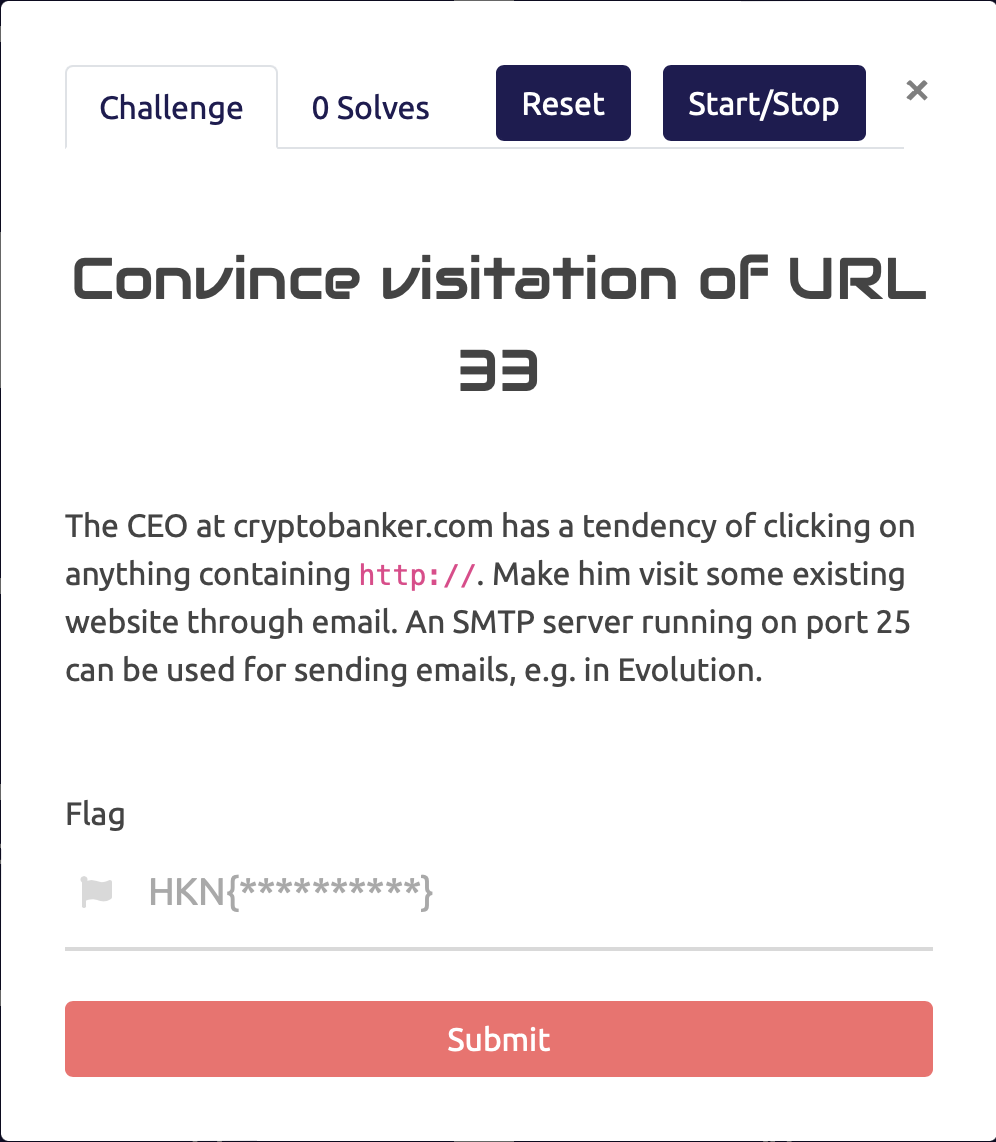
\includegraphics[scale=.4]{figures/flag-submission-modal.png}}
\caption{A challenge modal in Haaukins platform}
\label{fig}
\end{figure}
\newpage


\subsubsection{Flag}
 Flag is special secret string inserted into vulnerable application when building. Participants' goal is to reach hidden flags and submit them through web user interface shown given in Figure 3.1


\subsection{Overview}
 In general, an event can contain one or more labs, a lab can contain at least one or more challenges. Overview relation between different components can be observed by Figure 3.2
 
\begin{figure}[htbp]
\centerline{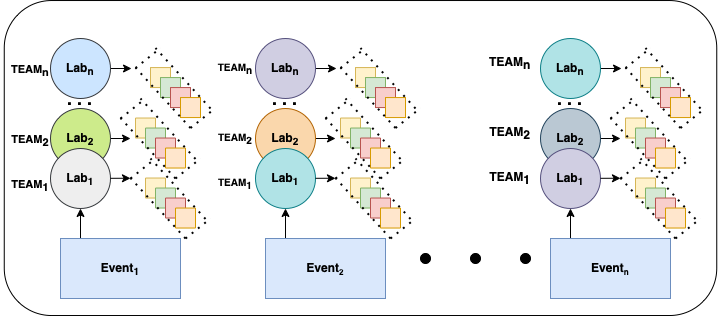
\includegraphics[scale=.5]{figures/relationship-diagram.png}}
\caption{The relationship between different components in Haaukins platform}
\label{fig}
\end{figure}
 
As shown in Figure 3.1, each lab consists of different challenges and a virtual machine for participants to use on browser. The virtual machine is generally Kali or Parrot, since they include wide range of cyber security tool. When a participant sign up the event, they automatically assign a lab which is completely isolated from other team's lab. All this automation does not require any extra step from the participant perspective. A challenge can be built up from one or more containers or with virtual machines directly. Since challenges can be deployed as containers, they are lightweight compared to virtual machines. It brings great flexibility and scaling when there is high number of participants. Although containerization is great to use, sometimes it is not possible to emulate scenarios where the vulnerability is related to Windows Operating System core functionality for instance "Buffer Overrun In RPC Interface Could Allow Code Execution"\footnote{https://docs.microsoft.com/en-us/security-updates/securitybulletins/2003/ms03-026}


\subsubsection{Golang}

Golang is a decent programming language developed by Google\footnote{https://en.wikipedia.org/wiki/Go_(programming_language)}. It provides built-in concurrency and fast processing capabilities. Haaukins platform is entirely written in Go programming language to benefit from built-in concurrency and huge community support. 
Golang is commonly used in system level automation tasks by large communities, some well-known projects written in Go are, Kubernetes, Docker, Prometheus, Terraform and many more. 
Due to its advantages compared to other languages, the platform is built entirely in Go language. 

\subsubsection{Virtual Box}

Virtual box is used as hypervisor to handle challenges on VM (Virtual Machine) and assigned VMs to the participants to the event. VMs are linked with Docker network interface to be able to attack vulnerable machines resides on same network. 
\subsubsection{Docker}

Main core part of Haaukins platform is Docker containerization technology, the platform automates process of managing docker containers. Docker is providing virtual networking by creating macvlan network\footnote{https://docs.docker.com/network/macvlan/} interfaces when used with virtual machine on browser mode. 
In case of virtual private networking (VPN) mode, Docker bridge network\footnote{https://docs.docker.com/network/bridge/} is used and network packets controlled with network tools such as iptables.
\begin{figure}[htbp]
\centerline{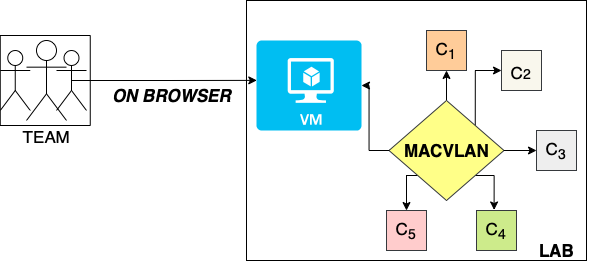
\includegraphics[scale=.4]{figures/macvlan-arch.png}}
\caption{Lab internals, macvlan connection }
\label{fig}
\end{figure}
In Figure 3.2, how a team is connected isolated lab environment with macvlan networks is shown. All challenges and VM is connected to common macvlan network to reach vulnerable machines. Team/Participant is connected on browser to customized virtual machine which includes cyber security tools, for instance operating system Kali\footnote{https://www.kali.org} or Parrot\footnote{https://www.parrot.com/en} The connection between user and virtual machine on browser is done by open source Apache Guacamole project.

\subsubsection{Apache Guacamole}\footnote{https://guacamole.apache.org}
Apache Guacamole provides stable connection to a virtual machine through browser. It removes necessity of installing additional software to participants' computer when joining an event running on Haaukins platform. 
All the steps are automated with Go programming language and it enables users to have a custom set of challenges. Haaukins platform can manage as many events as possible, limited to server resources (CPU, Memory). Each event can include different sets of challenges to hack, at the end of hacking, participants will receive dynamically generated flag. It means although challenges are same the flags will be unique per participants, which is generally not supported by other platforms. 

\subsection{Challenges}

Challenges in the platform is developed specifically for a course (e.g Network Security, Cryptography, Security Engineering) or company based training course to provide specialized learning experience. A challenge can be a docker container, a virtual machine or group of docker containers. Since challenges are created parallel to course syllabus, understanding conceptional topics becomes easy for participants. Therefore, the platform has been used at Aalborg University\footnote{https://www.en.aau.dk/education/master/cyber-security/},  Hogeschool Saxion\footnote{https://www.saxion.edu/programmes/bachelor/applied-computer-science} and Denmark Technical University (DTU)\footnote{https://www.compute.dtu.dk/english/continuing-education/master-of-cyber-security/study-program} in relative courses. 

\subsubsection{Deployment of Challenges}

Challenges, running in container(s), are deployed automatically to the platform in a micro service architecture approach. 

\begin{figure}[htbp]
\centerline{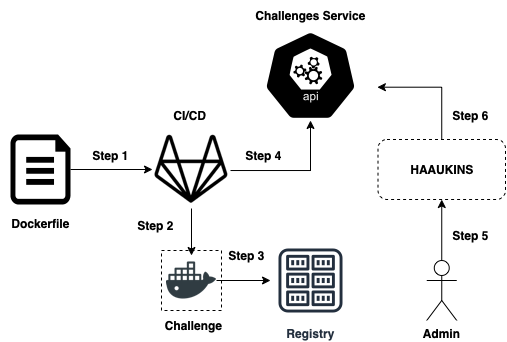
\includegraphics[scale=.6]{figures/challenge-deployment.png}}
\caption{Challenge deployment architecture diagram }
\label{fig}
\end{figure}
\newpage 
Figure 3.4 represents how a challenge is automatically deployed to the platform. The process does not include any human interaction after Step 1. 

In Step 1, challenge creator should define all components of a challenge to be running, which includes codes, framework, programming language and if required more information. Once, they have been defined in a simple Dockerfile\footnote{https://docs.docker.com/engine/reference/builder/} and pushed a repository (on Gitlab/Github), all other steps are automatically completed.  It brings great opportunity for other institutions to contribute the platform. Any institution can create challenges based on their requirement and shipped to Haaukins platform in one manual step. Indeed, the collaboration, between the universities who use Haaukins platform, is adequately increased. They decided to create a cluster of point where Haaukins can be scaled and improved even more with innovative challenges. 

In Step 2, Gitlab CI*\footnote{Continuous integration} builds and creates a Docker image\footnote{https://docs.docker.com/engine/reference/commandline/image/}, it provides a packed application which can run anywhere as long as Docker daemon exists. 

In Step 3, the created image is saved to a some kind of database with all content of the application. In case existence, it automatically updates existing image. 
In Step 4, a configuration file is pushed to a microservice which contains information about an exercise, for instance, image name, registry information, flag information and some metadata. 

In Step 5, in case a challenge is requested to be included in an event, Haaukins can pull and run it as shown in the Figure 3.4

In Step 6, an event organizer or instructor creates an event on administration page. 

\subsection{Virtual Private Network Access}
Extensive usage of the platform extended its target group with professional security engineers. Even though professional security engineers are in seek of bug bounty programs, they interested to play with the platform. Professionals do not like to play with a virtual machine on a browser with no internet connection. Instead, their preference is mostly to use their customised environment for real tough challenges exists on the platform. Therefore, Wireguard\footnote{https://www.wireguard.com} introduced to mitigate the problems of experienced users. It provides connectivity to challenges running on virtual network without using any virtual machine on browser.Compared to other existing platforms, virtual private network solution is different in Haaukins platform thanks to resilient Wireguard implementation. The platform is communicating with Wireguard service, which runs independently from the platform, to create requested clients from the platform. 
Additionally, VPN solution provides simultaneously access for a lab assigned to a team. A team up to four people can access and solve challenges at the same time. The default limit for a lab to be access at the same time is four.However, it is a configuration matter and can be adjusted according to need. 
Wireguard is special compared to OpenVPN, enormous improvements are introduced on ping time and throughput\cite{wireguard}.Therefore, Haaukins platform outperforms compared to other commercial e-Learning platforms. 


